\documentclass{../weeklyslides}

\addbibresource{../../References.bib}

\title[Weekly Report]{ECE 497: Special Project \\ Weekly Report}
\subtitle{Week 02}
\author{Alexander Lukens \and Karl Hallsby}
\institute{Illinois Institute of Technology}
\date{\today}

\begin{document}

\nocite{chipyard}

\begin{frame}
  \titlepage{}
\end{frame}

\section{What We Did}\label{sec:What_We_Did}
\begin{frame}
  \frametitle{\nameref*{sec:What_We_Did}}
  \begin{itemize}
  \item Set up Virtual machines to have similar environments.
  \item Clone the ChipYard repository.
  \item Build the toolchains required (Quite time-consuming)
  \item Followed documentation's example on how to generate a generic RISC-V chip.
  \item Used Verilator to simulate the default chip design.
    \begin{itemize}
    \item Ran all tests (\texttt{make run-asm-tests}) (Quite time consuming)
    \item Ran all benchmarks (\texttt{make run-bmark-tests})
    \item As expected, the default chip design passed all tests and benchmarks successfully.
    \end{itemize}
  \end{itemize}
\end{frame}

\section{What We Learned}\label{sec:What_We_Learned}
\begin{frame}
  \frametitle{\nameref*{sec:What_We_Learned}}
  \begin{itemize}
  \item \emph{Simulated} chip designs operate at O(\SI{1}{\kilo\hertz}).
    \begin{itemize}
    \item According to the documentation, these are significantly easier to debug.
    \end{itemize}
  \item \emph{FPGA-accelerated} chip designs operate at O(\SI{100}{\mega\hertz}).
    \begin{itemize}
    \item These are also significantly more difficult to debug.
    \item This speed is reached only when using FireSim (AWS).
    \item We believe this implies we can write out the Verilog to Alex's FPGA and test there, albeit more slowly.
    \end{itemize}
  \item \texttt{make run-asm-tests} runs all the instructions in the CPU design, ensuring ISA compliance.
  \item To get waveform outputs, run \texttt{make debug} when generating the simulated chip binary.
  \end{itemize}
\end{frame}

\begin{frame}
  \begin{itemize}
  \item The Chipyard built-in tests for simulations are sufficient to ensure complete RISC-V compliance of a custom SoC.
  \item Testing the entire ISA takes a significant amount of time, should only be completed when finalizing custom design, before FPGA implementation.
  \item There are many simulator options available. Significant options include \texttt{VERILATOR\_THREADS}, \texttt{make verilog}, \texttt{make run-binary-debug}
  \item Using \texttt{make verilog} to generate the design completely in verilog, the default design should be able to be synthesized on the FPGA board
  \end{itemize}
\end{frame}

\begin{frame}
  \begin{figure}
    \centering
    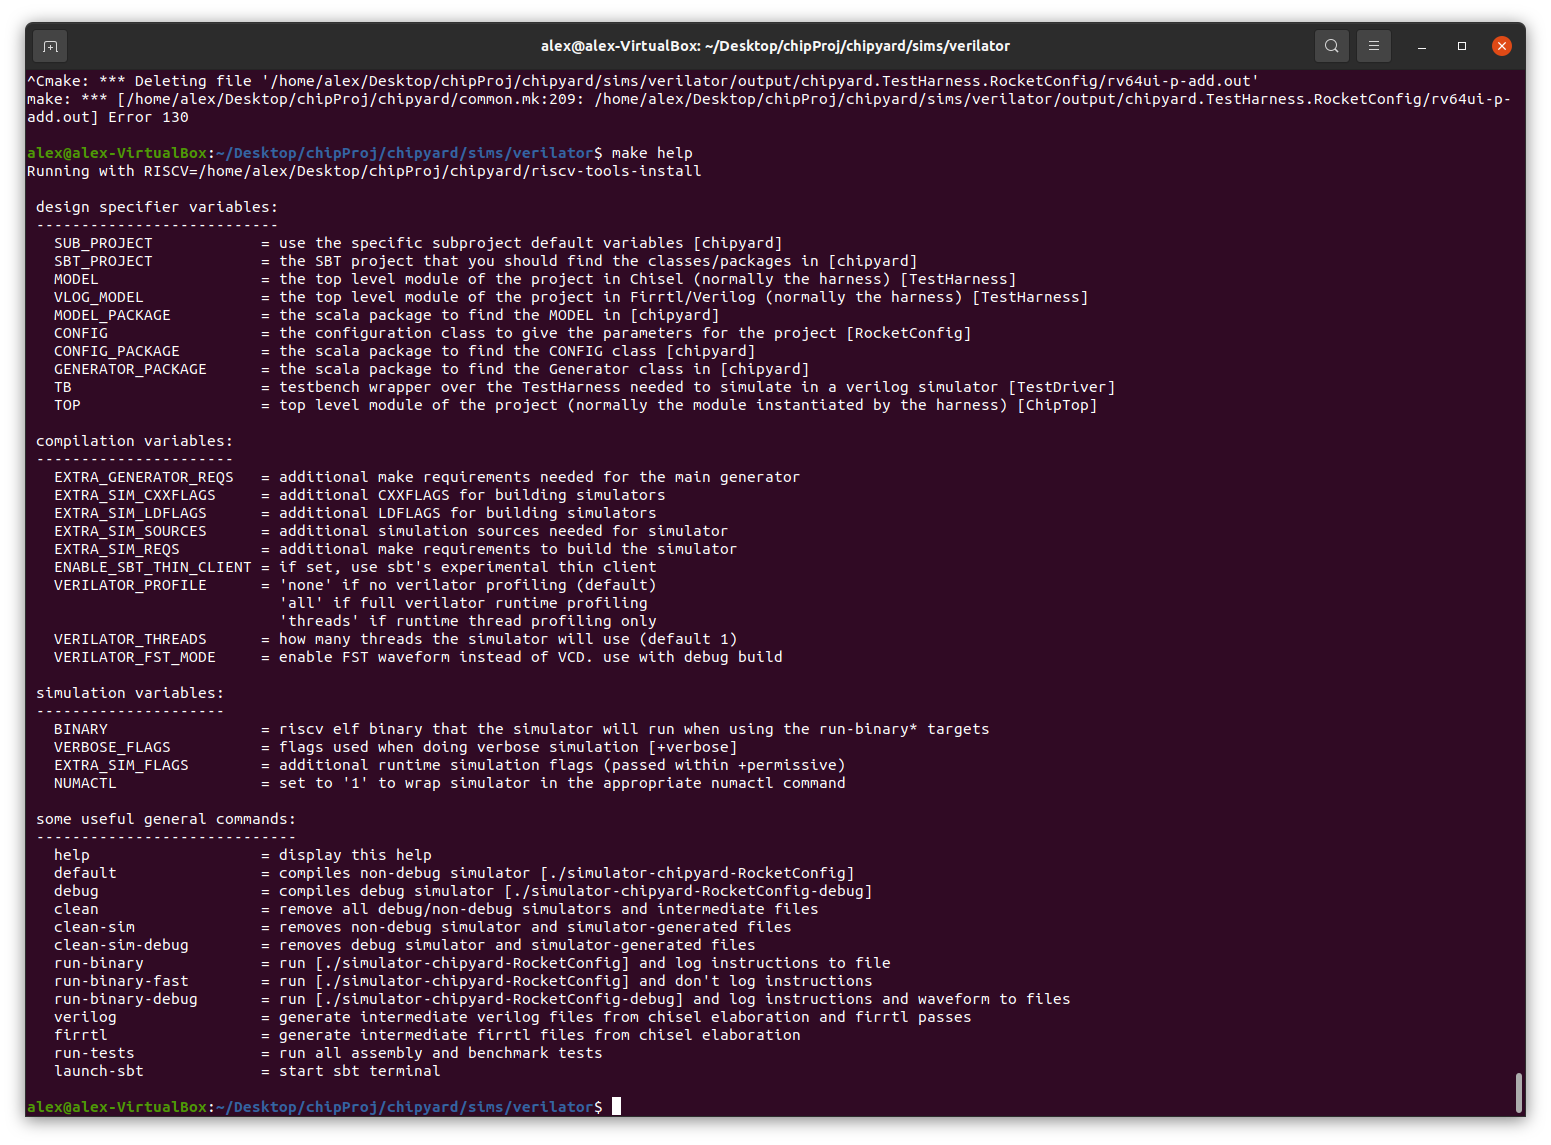
\includegraphics[width=1\linewidth]{./verilator_options.png}
    \caption{Chipyard Simulator Options and Flags}
    \label{fig:verilator-options}
  \end{figure}
\end{frame}

\section{Next Steps}\label{sec:Next_Steps}
\begin{frame}
  \frametitle{\nameref*{sec:Next_Steps}}
  \begin{itemize}
  \item Write the default chip out to Alex's FPGA and test.
  \item Use Scala/Chisel to generate a custom chip.
  \item Simulate the custom chip in software.
  \item Write the custom chip out to the FPGA.\@
  \end{itemize}
\end{frame}

\begin{frame}
  \frametitle{References}
  \printbibliography[heading=bibintoc]{}
\end{frame}

\end{document}

%%% Local Variables:
%%% mode: latex
%%% TeX-master: t
%%% End:
